%\iffalse meta-comment
%Copyright (c) 2018 Matthew Scroggs
%
%Permission is hereby granted, free of charge, to any person obtaining a copy
%of this software and associated documentation files (the "Software"), to deal
%in the Software without restriction, including without limitation the rights
%to use, copy, modify, merge, publish, distribute, sublicense, and/or sell
%copies of the Software, and to permit persons to whom the Software is
%furnished to do so, subject to the following conditions:
%
%The above copyright notice and this permission notice shall be included in all
%copies or substantial portions of the Software.
%
%THE SOFTWARE IS PROVIDED "AS IS", WITHOUT WARRANTY OF ANY KIND, EXPRESS OR
%IMPLIED, INCLUDING BUT NOT LIMITED TO THE WARRANTIES OF MERCHANTABILITY,
%FITNESS FOR A PARTICULAR PURPOSE AND NONINFRINGEMENT. IN NO EVENT SHALL THE
%AUTHORS OR COPYRIGHT HOLDERS BE LIABLE FOR ANY CLAIM, DAMAGES OR OTHER
%LIABILITY, WHETHER IN AN ACTION OF CONTRACT, TORT OR OTHERWISE, ARISING FROM,
%OUT OF OR IN CONNECTION WITH THE SOFTWARE OR THE USE OR OTHER DEALINGS IN THE
%SOFTWARE.
%\fi

% \lstinline{tikz-truchet} is a package for \LaTeX{} that draws Truchet tiles,
% as features in the article \emph{Too good to be Truchet} by Colin Beveridge\footnote{Chalkdust Magazine issue 08, Autumn 2018,
% \url{http://chalkdustmagazine.com/features/too-good-to-be-truchet/}}.
%\iffalse
%<*documentation>
\documentclass{article}
\usepackage{tikz-truchet}
\usepackage{doc}
\usepackage{listings}
\usepackage{url}
\usepackage{hyperref}
\lstset{basicstyle=\ttfamily\footnotesize,commentstyle=\color{red},language=[LaTeX]TeX}
\title{tikz-truchet v\input{VERSION}}
\author{Matthew W.~Scroggs}
\begin{document}
\maketitle
    \DocInput{tikz-truchet.dtx}
\end{document}
%</documentation>
%\fi
%
%\iffalse
%<*truchet>
\NeedsTeXFormat{LaTeX2e}
\ProvidesPackage{tikz-truchet}[2019/02/12 tikz-truchet]

\RequirePackage{tikz}
\RequirePackage{ifthen}

%\fi
% Before starting, I recommend setting the following tikz options to make your pictures look nicer:
%\begin{lstlisting}
\tikzset{x=2cm,y=2cm,line cap=round,line join=round, every picture}
%\end{lstlisting}
%
% \section{Squares}
% \DescribeMacro{\truchetsquare}
% You can draw square Truchet tile using the command \lstinline{\truchetsquare}.
% The following code will produce the output below.
%\iffalse
%<*example>
%\fi
\begin{lstlisting}

\begin{tikzpicture}
  \truchetsquare{b}{w}{b}{w}{b}
\end{tikzpicture}
\end{lstlisting}
%\iffalse
%</example>
%\fi
% \begin{center}
% \begin{tikzpicture}
%   \truchetsquare{b}{w}{b}{w}{b}
% \end{tikzpicture}
% \end{center}
% The five inputs of the command are the colour (\lstinline{b} or \lstinline{w}) at the centre, the North East, North West, South West,
% and South East corners (in that order)
%
% You can a square bracketed input to move the tiles. The tiles are 1 unit wide.
%\iffalse
%<*example>
%\fi
\begin{lstlisting}
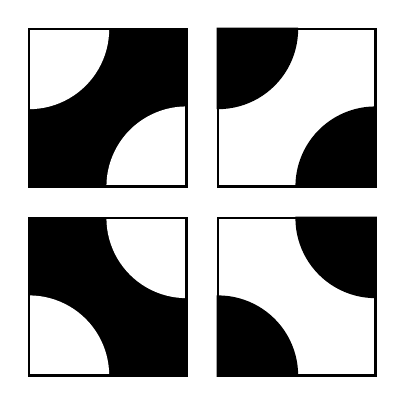
\begin{tikzpicture}
  \truchetsquare{b}{w}{b}{w}{b}
  \truchetsquare[(1.2,0)]{w}{b}{w}{b}{w}
  \truchetsquare[(0,-1.2)]{b}{b}{w}{b}{w}
  \truchetsquare[(1.2,-1.2)]{w}{w}{b}{w}{b}
\end{tikzpicture}
\end{lstlisting}
%\iffalse
%</example>
%\fi
% \begin{center}
% \begin{tikzpicture}
%   \truchetsquare{b}{w}{b}{w}{b}
%   \truchetsquare[(1.2,0)]{w}{b}{w}{b}{w}
%   \truchetsquare[(0,-1.2)]{b}{b}{w}{b}{w}
%   \truchetsquare[(1.2,-1.2)]{w}{w}{b}{w}{b}
% \end{tikzpicture}
% \end{center}
%
%\iffalse
\newcommand{\truchetsquare}[6][(0,0)]{
  \begin{scope}[shift={#1}]
    \ifthenelse{\equal{#2}{b}}{
        \draw[black,fill=black] (0,0) rectangle (1,1);
    }{
        \draw[white,fill=white] (0,0) rectangle (1,1);
    }
    \ifthenelse{\equal{#3}{#2}}{}{
        \ifthenelse{\equal{#3}{b}}{
            \draw [black,fill=black,domain=0:90,line width=1pt] plot ({0.5*cos(\x)}, {1-0.5*sin(\x)}) -- (0,1) -- cycle;
        }{
            \draw [white,fill=white,domain=0:90,line width=1pt] plot ({0.5*cos(\x)}, {1-0.5*sin(\x)}) -- (0,1) -- cycle;
        }
    }
    \ifthenelse{\equal{#4}{#2}}{}{
        \ifthenelse{\equal{#4}{b}}{
            \draw [black,fill=black,domain=0:90,line width=1pt] plot ({1-0.5*cos(\x)}, {1-0.5*sin(\x)}) -- (1,1) -- cycle;
        }{
            \draw [white,fill=white,domain=0:90,line width=1pt] plot ({1-0.5*cos(\x)}, {1-0.5*sin(\x)}) -- (1,1) -- cycle;
        }
    }
    \ifthenelse{\equal{#5}{#2}}{}{
        \ifthenelse{\equal{#5}{b}}{
            \draw [black,fill=black,domain=0:90,line width=1pt] plot ({1-0.5*cos(\x)}, {0.5*sin(\x)}) -- (1,0) -- cycle;
        }{
            \draw [white,fill=white,domain=0:90,line width=1pt] plot ({1-0.5*cos(\x)}, {0.5*sin(\x)}) -- (1,0) -- cycle;
        }
    }
    \ifthenelse{\equal{#6}{#2}}{}{
        \ifthenelse{\equal{#6}{b}}{
            \draw [black,fill=black,domain=0:90,line width=1pt] plot ({0.5*cos(\x)}, {0.5*sin(\x)}) -- (0,0) -- cycle;
        }{
            \draw [white,fill=white,domain=0:90,line width=1pt] plot ({0.5*cos(\x)}, {0.5*sin(\x)}) -- (0,0) -- cycle;
        }
    }
    \draw[black,line width=1pt] (0,0) rectangle (1,1);
  \end{scope}
}
%\fi 
% 
% \DescribeMacro{\diagonalsquare}
% The command \lstinline{\diagonalsquare} can be used to draw a square tile that is half white and half black along a diagonal.
%\iffalse
%<*example>
%\fi
\begin{lstlisting}
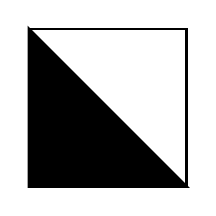
\begin{tikzpicture}
  \diagonalsquare{x}{w}{x}{b}
\end{tikzpicture}
\end{lstlisting}
%\iffalse
%</example>
%\fi 
% \begin{center}
% \begin{tikzpicture}
% \diagonalsquare{x}{w}{x}{b}
% \end{tikzpicture}
% \end{center}
% The four inputs are the color (\lstinline{b} or \lstinline{w}), or \lstinline{x} if the colour changes at that corner, of
% the North East, North West, South West, and South East corners (in that order).
%
% \DescribeMacro{\tileA}
% \DescribeMacro{\tileB}
% \DescribeMacro{\tileC}
% \DescribeMacro{\tileD}
% There are only five such tiles. They can be created using the convenience functions
% \lstinline{\tileA},
% \lstinline{\tileB},
% \lstinline{\tileC}, and
% \lstinline{\tileD}.
%\iffalse
%<*example>
%\fi
\begin{lstlisting}
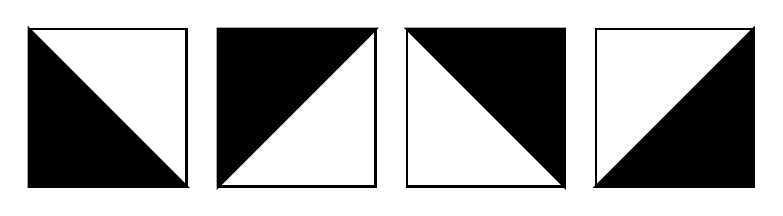
\begin{tikzpicture}
  \tileA
  \tileB[(1.2,0)]
  \tileC[(2.4,0)]
  \tileD[(3.6,0)]
\end{tikzpicture}
\end{lstlisting}
%\iffalse
%</example>
%\fi 
% \begin{center}
% \begin{tikzpicture}
%  \tileA
%  \tileB[(1.2,0)]
%  \tileC[(2.4,0)]
%  \tileD[(3.6,0)]
% \end{tikzpicture}
% \end{center}
% 
%\iffalse
\newcommand{\diagonalsquare}[5][(0,0)]{
  \begin{scope}[shift={#1}]
    \draw[white,fill=white] (0,0) rectangle (1,1);
    \ifthenelse{\equal{#2}{b}}{
        \draw [black,fill=black,line width=1pt] (0,0) -- (0,1) -- (1,1) -- cycle;
    }{}
    \ifthenelse{\equal{#3}{b}}{
        \draw [black,fill=black,line width=1pt] (0,1) -- (1,1) -- (1,0) -- cycle;
    }{}
    \ifthenelse{\equal{#4}{b}}{
        \draw [black,fill=black,line width=1pt] (1,1) -- (1,0) -- (0,0) -- cycle;
    }{}
    \ifthenelse{\equal{#5}{b}}{
        \draw [black,fill=black,line width=1pt] (1,0) -- (0,0) -- (0,1) -- cycle;
    }{}
    \draw[black,line width=1pt] (0,0) rectangle (1,1);
  \end{scope}
}

\newcommand{\tileA}[1][(0,0)]{\diagonalsquare[#1]{x}{w}{x}{b}}
\newcommand{\tileB}[1][(0,0)]{\diagonalsquare[#1]{b}{x}{w}{x}}
\newcommand{\tileC}[1][(0,0)]{\diagonalsquare[#1]{x}{b}{x}{w}}
\newcommand{\tileD}[1][(0,0)]{\diagonalsquare[#1]{w}{x}{b}{x}}

%\fi
%
% \section{Hexagons}
% To draw hexagonal Truchet tiles, you can use the commands \lstinline{\truchethex} and \lstinline{\truchetsplithex}.
%
% \DescribeMacro{\truchethex}
% The command \lstinline{\truchethex} takes 7 inputs: the colour (\lstinline{b} or \lstinline{w}) at the
% centre, then all the corners starting at the top left and going clockwise. Again an argument can be passed in square
% brackets to move the tile.
%\iffalse
%<*example>
%\fi
\begin{lstlisting}
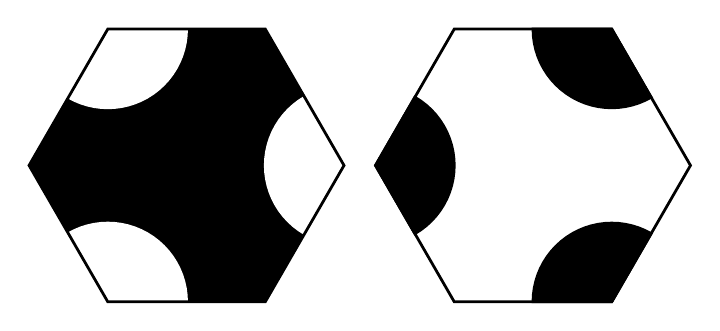
\begin{tikzpicture}
  \truchethex{b}{w}{b}{w}{b}{w}{b}
  \truchethex[(2.2,0)]{w}{w}{b}{w}{b}{w}{b}
\end{tikzpicture}
\end{lstlisting}
%\iffalse
%</example>
%\fi 
% \begin{center}
% \begin{tikzpicture}
%  \truchethex{b}{w}{b}{w}{b}{w}{b}
%  \truchethex[(2.2,0)]{w}{w}{b}{w}{b}{w}{b}
% \end{tikzpicture}
% \end{center}
%
% \DescribeMacro{\truchetsplithex}
% The command \lstinline{\truchetsplithex} draws a Truchet tile split in half like the following.
%\iffalse
%<*example>
%\fi
\begin{lstlisting}
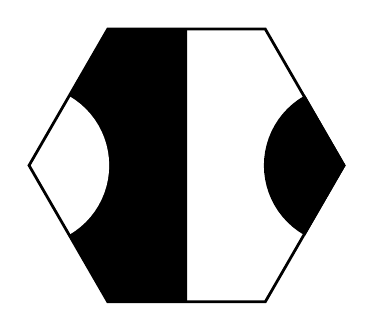
\begin{tikzpicture}
  \truchetsplithex
\end{tikzpicture}
\end{lstlisting}
%\iffalse
%</example>
%\fi 
% \begin{center}
% \begin{tikzpicture}
%  \truchetsplithex
% \end{tikzpicture}
% \end{center}
% 
% \DescribeEnv{rotatehex}
% The environment \lstinline{rotatehex} can be used to rotate a hexagonal tile about its centre. The angle should be given in degrees.
% 
%\iffalse
%<*example>
%\fi
\begin{lstlisting}
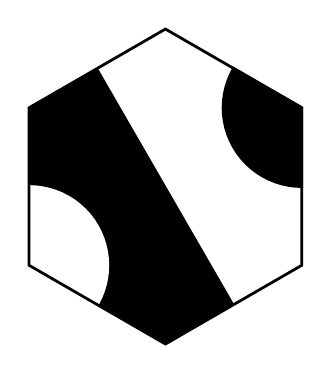
\begin{tikzpicture}
  \begin{rotatehex}{30}
    \truchetsplithex
  \end{rotatehex}
\end{tikzpicture}
\end{lstlisting}
%\iffalse
%</example>
%\fi 
% \begin{center}
% \begin{tikzpicture}
%  \begin{rotatehex}{30}
%    \truchetsplithex
%  \end{rotatehex}
%  \begin{rotatehex}{30}
%    \truchetsplithex
%  \end{rotatehex}
% \end{tikzpicture}
% \end{center}
% 
%\iffalse
\newcommand{\truchetsplithex}[1][(0,0)]{
  \begin{scope}[shift={#1}]
    \draw[white,fill=white] (0,0) -- (1,0) -- (1.5,0.866) -- (1,1.732) -- (0,1.732) -- (-0.5,0.866) -- cycle;
    \draw[black,fill=black] (0,0) -- (.5,0) -- (.5,1.732) -- (0,1.732) -- (-0.5,0.866) -- cycle;
    \draw [black,fill=black,domain=120:240,line width=1pt] plot ({1.5+0.5*cos(\x)}, {0.866+0.5*sin(\x)}) -- (1.5,0.866) -- cycle;
    \draw [white,fill=white,domain=-60:60,line width=1pt] plot ({-0.5+0.5*cos(\x)}, {0.866+0.5*sin(\x)}) -- (-0.5,0.866) -- cycle;
    \draw[black,line width=1pt] (0,0) -- (1,0) -- (1.5,0.866) -- (1,1.732) -- (0,1.732) -- (-0.5,0.866) -- cycle;
  \end{scope}
}

\newcommand{\truchethex}[8][(0,0)]{
  \begin{scope}[shift={#1}]
    \ifthenelse{\equal{#2}{b}}{
        \draw[black,fill=black] (0,0) -- (1,0) -- (1.5,0.866) -- (1,1.732) -- (0,1.732) -- (-0.5,0.866) -- cycle;
    }{
        \draw[white,fill=white] (0,0) -- (1,0) -- (1.5,0.866) -- (1,1.732) -- (0,1.732) -- (-0.5,0.866) -- cycle;
    }
    \ifthenelse{\equal{#3}{#2}}{}{
        \ifthenelse{\equal{#3}{b}}{
            \draw [black,fill=black,domain=240:360,line width=1pt] plot ({0.5*cos(\x)}, {1.732+0.5*sin(\x)}) -- (0,1.732) -- cycle;
        }{
            \draw [white,fill=white,domain=240:360,line width=1pt] plot ({0.5*cos(\x)}, {1.732+0.5*sin(\x)}) -- (0,1.732) -- cycle;
        }
    }
    \ifthenelse{\equal{#4}{#2}}{}{
        \ifthenelse{\equal{#4}{b}}{
            \draw [black,fill=black,domain=180:300,line width=1pt] plot ({1+0.5*cos(\x)}, {1.732+0.5*sin(\x)}) -- (1,1.732) -- cycle;
        }{
            \draw [white,fill=white,domain=180:300,line width=1pt] plot ({1+0.5*cos(\x)}, {1.732+0.5*sin(\x)}) -- (1,1.732) -- cycle;
        }
    }
    \ifthenelse{\equal{#5}{#2}}{}{
        \ifthenelse{\equal{#5}{b}}{
            \draw [black,fill=black,domain=120:240,line width=1pt] plot ({1.5+0.5*cos(\x)}, {0.866+0.5*sin(\x)}) -- (1.5,0.866) -- cycle;
        }{
            \draw [white,fill=white,domain=120:240,line width=1pt] plot ({1.5+0.5*cos(\x)}, {0.866+0.5*sin(\x)}) -- (1.5,0.866) -- cycle;
        }
    }
    \ifthenelse{\equal{#6}{#2}}{}{
        \ifthenelse{\equal{#6}{b}}{
            \draw [black,fill=black,domain=60:180,line width=1pt] plot ({1+0.5*cos(\x)}, {0.5*sin(\x)}) -- (1,0) -- cycle;
        }{
            \draw [white,fill=white,domain=60:180,line width=1pt] plot ({1+0.5*cos(\x)}, {0.5*sin(\x)}) -- (1,0) -- cycle;
        }
    }
    \ifthenelse{\equal{#7}{#2}}{}{
        \ifthenelse{\equal{#7}{b}}{
            \draw [black,fill=black,domain=0:120,line width=1pt] plot ({0.5*cos(\x)}, {0.5*sin(\x)}) -- (0,0) -- cycle;
        }{
            \draw [white,fill=white,domain=0:120,line width=1pt] plot ({0.5*cos(\x)}, {0.5*sin(\x)}) -- (0,0) -- cycle;
        }
    }
    \ifthenelse{\equal{#8}{#2}}{}{
        \ifthenelse{\equal{#8}{b}}{
            \draw [black,fill=black,domain=-60:60,line width=1pt] plot ({-0.5+0.5*cos(\x)}, {0.866+0.5*sin(\x)}) -- (-0.5,0.866) -- cycle;
        }{
            \draw [white,fill=white,domain=-60:60,line width=1pt] plot ({-0.5+0.5*cos(\x)}, {0.866+0.5*sin(\x)}) -- (-0.5,0.866) -- cycle;
        }
    }
    \draw[black,line width=1pt] (0,0) -- (1,0) -- (1.5,0.866) -- (1,1.732) -- (0,1.732) -- (-0.5,0.866) -- cycle;
  \end{scope}
}


\newenvironment{rotatehex}[1]{
    \begin{scope}[shift={(0.5,0.866)}]
        \begin{scope}[rotate=#1]
            \begin{scope}[shift={(-0.5,-0.866)}]
}{
            \end{scope}
        \end{scope}
    \end{scope}
}

%\fi
%
% \section{Cubes}
% \DescribeMacro{\truchetcube}
% The command \lstinline{\truchetcube} can be used to draw Cubes with differently coloured faces.
% The six inputs of the command are the colour (\lstinline{b} or \lstinline{w}) of the
% bottom, front, right, back, left, and top faces of the cube (in that order).
%\iffalse
%<*example>
%\fi
\begin{lstlisting}
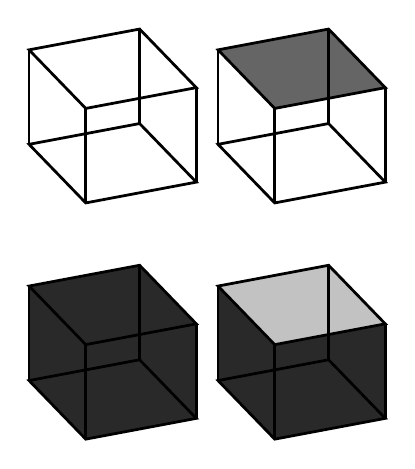
\begin{tikzpicture}[x=1.2cm,y=1.2cm]
\truchetcube{w}{w}{w}{w}{w}{w}
\truchetcube[(0,-3cm)]{b}{b}{b}{b}{b}{b}
\truchetcube[(2.4cm,0)]{w}{w}{w}{w}{w}{b}
\truchetcube[(2.4cm,-3cm)]{b}{b}{b}{b}{b}{w}
\end{tikzpicture}
\end{lstlisting}
%\iffalse
%</example>
%\fi 
% \begin{center}
% \begin{tikzpicture}[x=1.2cm,y=1.2cm]
% \truchetcube{w}{w}{w}{w}{w}{w}
% \truchetcube[(0,-3cm)]{b}{b}{b}{b}{b}{b}
% \truchetcube[(2.4cm,0)]{w}{w}{w}{w}{w}{b}
% \truchetcube[(2.4cm,-3cm)]{b}{b}{b}{b}{b}{w}
% \end{tikzpicture}
% \end{center}
%\iffalse

\newcommand{\truchetcube}[7][(0,0)]{
  \begin{scope}[shift={#1}]
    %1.17,0.22
    %-0.38,0.67
    \coordinate (A) at (0,0);
    \coordinate (B) at (1.17,0.22);
    \coordinate (C) at (0.57,0.84);
    \coordinate (D) at (-0.6,0.62);
    \coordinate (E) at (0,1);
    \coordinate (F) at (1.17,1.22);
    \coordinate (G) at (0.57,1.84);
    \coordinate (H) at (-0.6,1.62);
    %faces
    \ifthenelse{\equal{#2}{b}}
    {\fill[fill=black,fill opacity=0.6] (A) -- (B) -- (C) -- (D) -- cycle;}
    {\fill[fill=white,fill opacity=0.6] (A) -- (B) -- (C) -- (D) -- cycle;}
    \ifthenelse{\equal{#3}{b}}
    {\fill[fill=black,fill opacity=0.6] (A) -- (B) -- (F) -- (E) -- cycle;}
    {\fill[fill=white,fill opacity=0.6] (A) -- (B) -- (F) -- (E) -- cycle;}
    \ifthenelse{\equal{#4}{b}}
    {\fill[fill=black,fill opacity=0.6] (B) -- (C) -- (G) -- (F) -- cycle;}
    {\fill[fill=white,fill opacity=0.6] (B) -- (C) -- (G) -- (F) -- cycle;}
    \ifthenelse{\equal{#5}{b}}
    {\fill[fill=black,fill opacity=0.6] (C) -- (D) -- (H) -- (G) -- cycle;}
    {\fill[fill=white,fill opacity=0.6] (C) -- (D) -- (H) -- (G) -- cycle;}
    \ifthenelse{\equal{#6}{b}}
    {\fill[fill=black,fill opacity=0.6] (D) -- (A) -- (E) -- (H) -- cycle;}
    {\fill[fill=white,fill opacity=0.6] (D) -- (A) -- (E) -- (H) -- cycle;}
    \ifthenelse{\equal{#7}{b}}
    {\fill[fill=black,fill opacity=0.6] (E) -- (F) -- (G) -- (H) -- cycle;}
    {\fill[fill=white,fill opacity=0.6] (E) -- (F) -- (G) -- (H) -- cycle;}
    %edges
    \draw[black,line width=1pt] (A) -- (B) -- (C) -- (D) -- cycle;
    \draw[black,line width=1pt] (E) -- (F) -- (G) -- (H) -- cycle;
    \draw[black,line width=1pt] (A) -- (E);
    \draw[black,line width=1pt] (B) -- (F);
    \draw[black,line width=1pt] (C) -- (G);
    \draw[black,line width=1pt] (D) -- (H);
  \end{scope}
}

%</truchet>
%\fi
